\documentclass{beamer}
\usepackage[utf8]{inputenc}
\usepackage[T1]{fontenc}
\usepackage{graphicx}
\usepackage{tcolorbox}
\usepackage{hyperref}
\hypersetup{
    colorlinks=true,
    linkcolor=pink,
    urlcolor=cyan,
    urlbordercolor=cyan,
}
\graphicspath{ {./images/} }

\usetheme{Arguelles}

\title{Tutorial 8}
\subtitle{CS3241 Computer Graphics (AY23/24)}
\date{\today}
\author{Wong Pei Xian}
\institute[]{\email{e0389023@u.nus.edu}}

\begin{document}

\frame[plain]{\titlepage}

\section{Question 1}

\begin{frame}
    \frametitle{Question 1}

    \vspace{1em}
    Given a plane, whose equation is $2x + 4y + 4z - 6 = 0$, 
    and a ray, whose origin is $[2, 0, -5]^T$ and its direction is $[1, 2, 3]^T$:

    \begin{enumerate}
        \item Calculate the location where the ray intersects the plane.
        \item Compute the normalized surface normal vector at the intersection point.
    \end{enumerate}

\end{frame}

\begin{frame}
    \frametitle{Point of intersection}

    \begin{tcolorbox}
        Equation of ray: \\
        \begin{equation*}
            [2, 0, -5]^T + k[1, 2, 3]^T = [2 + k, 2k, -5 +3k]^T
        \end{equation*}
    \end{tcolorbox}

    \begin{eqnarray*}
        2(2 + k) + 4(2k) + 4(-5 + 3k) - 6 &= 0\\
        22k &= 22\\
        k &= 1\\
    \end{eqnarray*}

\end{frame}

\begin{frame}
    \frametitle{Normalized surface normal vector}

    \begin{tcolorbox}
        Equation of plane: \\
        \begin{equation*}
            2x + 4y + 4z - 6 = 0 \Rightarrow n \cdot(r - r_0) = 0
        \end{equation*}
    \end{tcolorbox}

    \begin{equation*}
        n = \text{norm} \left( \begin{matrix} 2 \\ 4 \\ 4 \end{matrix} \right) = 
            \left[ \begin{matrix} 2 \\ 4 \\ 4 \end{matrix} \right] \times \frac{1}{\sqrt{2^2 + 4^2 + 4^2}} = 
            \left[ \begin{matrix} 1/3 \\ 2/3 \\ 2/3 \end{matrix} \right]
    \end{equation*}

\end{frame}

\section{Question 2}

\begin{frame}
    \frametitle{Question 2}
    In Whitted Ray Tracing, when a ray $P(t) = O + t D$ is being intersected with an 
    opaque sphere, we often consider only the intersection at the smaller $t$ value. 
    In what situation should we consider the intersection at the larger $t$ value? 

\end{frame}

\begin{frame}
    \frametitle{Possible answer: Camera is inside sphere}

    \begin{center}
        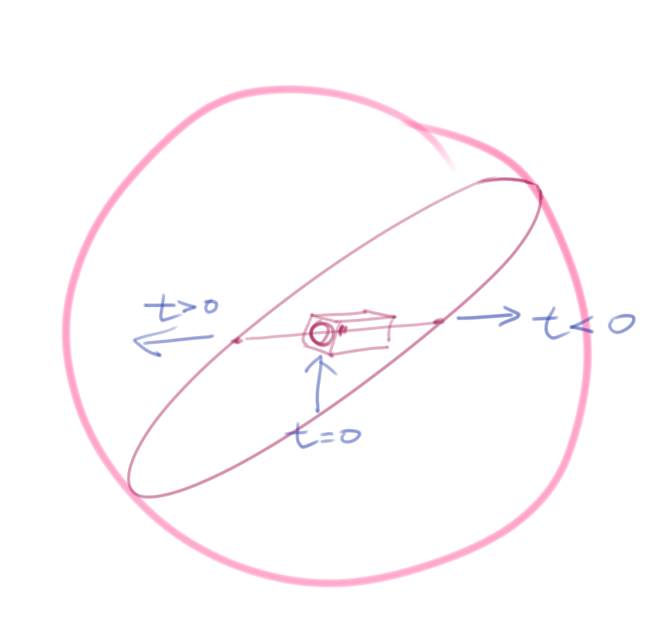
\includegraphics[scale=0.6]{q2.png}
    \end{center}

\end{frame}

\section{Question 3}

\begin{frame}
    \frametitle{Question 3}

    Suppose there is an enclosed scene, where all surfaces are \textbf{opaque} and have materials 
    that have both diffuse and specular components. There are \textbf{two point light sources} in the scene. 

    \vspace{1em}
    Assuming we want to render a \textbf{200x100 pixels} image of the scene using Whitted Ray Tracing, 
    with \textbf{three levels of recursion}, what would be the total number of rays that have to be shot?
\end{frame}

\begin{frame}
    \frametitle{Approach}

    For each pixel ($\times 20000$ pixels) per recursion:

    \begin{itemize}
        \item 2 shadow rays
        \item Reflected view ray (if recursion level $<3$)
        \item NO refracted view ray (\textbf(all surfaces are opaque!))
    \end{itemize}

    There are 1 primary set of rays, and 3 sets of reflected rays.\\

    Hence the total number of rays per pixel: $3 (1 + 3) = \mathbf{12}$.\\

    Total number of rays $= 12 \times 200 \times 100 = 240000$.

\end{frame}

\section{Question 4}

\begin{frame}
    \frametitle{Question 4}
    Explain why Whitted Ray Tracing cannot produce color bleeding effects 
    (diffuse-to-diffuse reflection).
\end{frame}

\begin{frame}
    \frametitle{Local illumination vs Global illumination}

    Local illumination only accumulates light from \textbf{direct light sources}.\\
    \textit{We only shoot shadow rays towards the light sources.}

    \vspace{1em}

    Global illumination accumulates light via \textcolor{teal}{\textbf{secondary light rays}}
    shot in \textbf{all directions} to collect light from diffuse surfaces.

\end{frame}

\begin{frame}
    \frametitle{Local illumination}

    Illustration with whitted ray tracing (green surface is diffuse):
    \begin{center}
        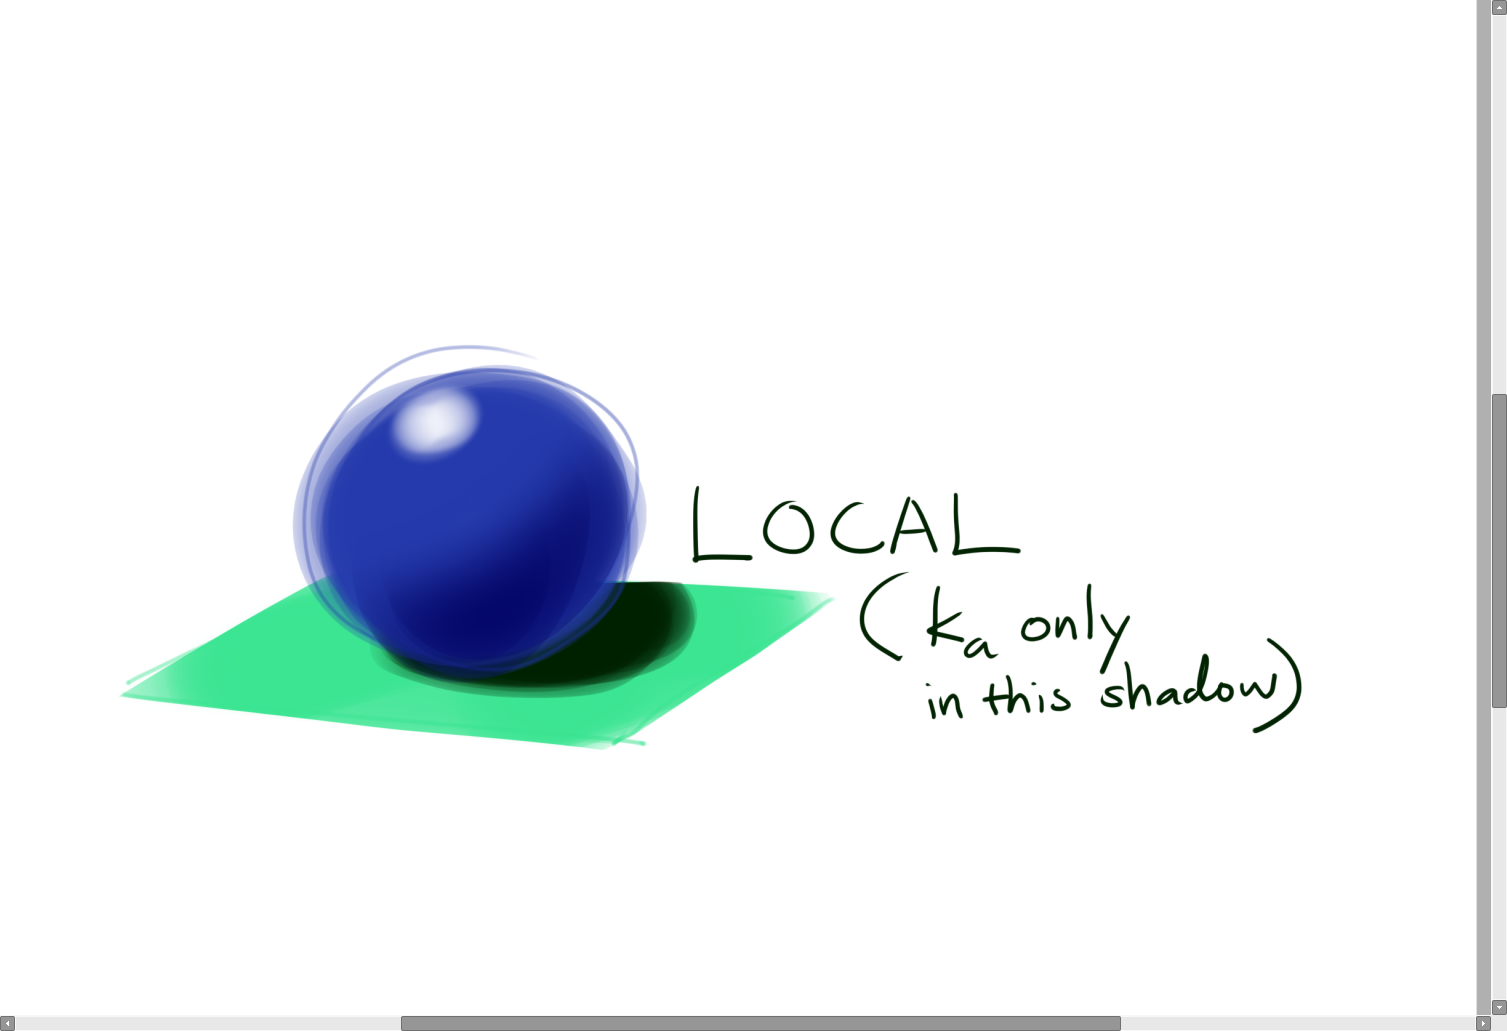
\includegraphics[scale=0.3]{local.png}
    \end{center}

\end{frame}

\begin{frame}
    \frametitle{Global illumination}

    Illustration with global illumination (e.g. path tracing, green surface still diffuse):
    \begin{center}
        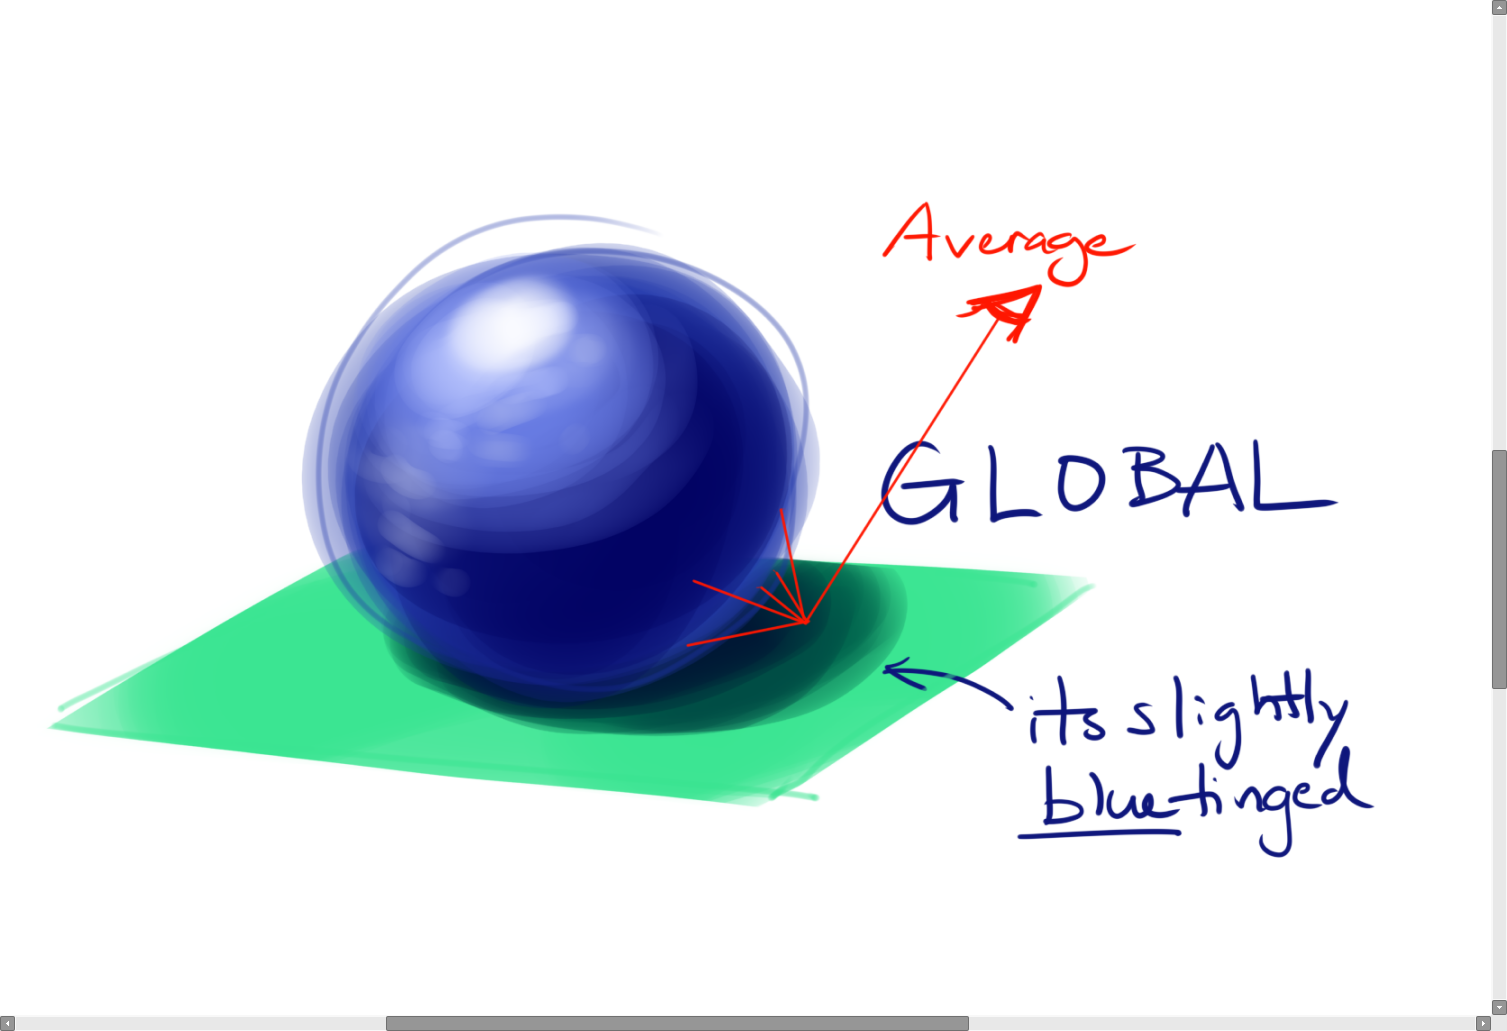
\includegraphics[scale=0.3]{global.png}
    \end{center}

\end{frame}

\section{Question 5}

\begin{frame}
    \frametitle{Question 5}
    Explain how the use of bounding volumes can accelerate ray tracing.
\end{frame}

\begin{frame}
    \frametitle{Fast elimination}

    \begin{center}
        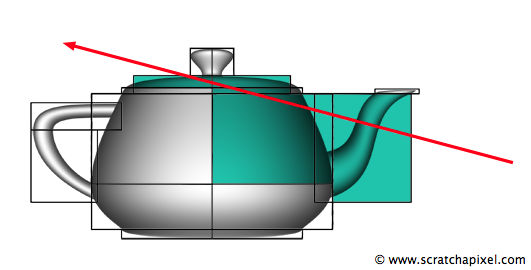
\includegraphics[scale=0.6]{bbox.png}
    \end{center}

\end{frame}

\begin{frame}
    \frametitle{What's the most expensive part of raytracing?}

    \textbf{Computing intersections.} \\
    \textit{e.g. How do you determine at which point does a ray intersect a parametric surface?}

    \vspace{1em}

    \begin{tcolorbox}
        By carving up our object into \textbf{bounding volumes} which the part of the object
        is contained within, we can \textbf{compute intersections with the bounding volume} instead. \\

        If miss: reject.\\
        If intersect: do actual intersection computation with surface.
    \end{tcolorbox}

\end{frame}

\section{Question 6}

\begin{frame}
    \frametitle{Question 6}
    Give two criteria for choosing a bounding volume shape for ray tracing acceleration. 
    What 3D shape(s) fulfill these criteria?
\end{frame}

\begin{frame}
    \frametitle{Some types}

    \begin{center}
        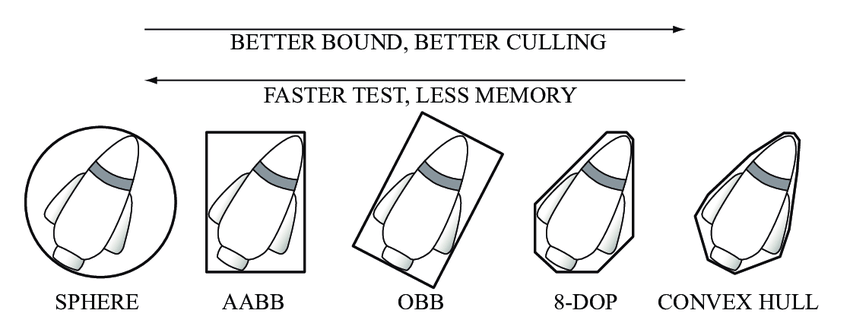
\includegraphics[scale=0.3]{best-to-worst-bb.png}
    \end{center}

\end{frame}

\begin{frame}
    \frametitle{Criteria}

    \begin{enumerate}
        \item Must enclose each object as tightly as possible
        \item Efficient to compute intersection with ray.
    \end{enumerate}

\end{frame}

\begin{frame}
    \frametitle{When is AABB bad?}

    e.g. compare AABB with OBB.

    \begin{tcolorbox}
        May not be a tight bounding volume for object shapes that are elongated and oriented diagonally.
    \end{tcolorbox}

\end{frame}


\begin{frame}[plain,standout]
    \AlegreyaExtraBold \LARGE
    Attendance taking
\end{frame}

\ThankYou
\begin{frame}[plain,standout]
    Thanks! Get the slides here after the tutorial.\\
    \vspace{2em}
    \scalebox{3}{\faGithub}\par\bigskip
    \url{https://trxe.github.io/cs3241-notes}
\end{frame}

\end{document}